\documentclass[14pt]{extarticle}
\input{external/preamble-latex-cools.tex}
\begin{document}
\begin{project}{Actividad de cierre}{Rosas para compartir.}{cool-rosasParaCompartir}%
Clare tiene 14 rosas. Quiere darle 2 rosas a cada una de sus profesoras. ¿A cuántas profesoras les puede dar rosas?%
\par
Escribe una ecuación de multiplicación y una ecuación de división que representen la situación. Usa símbolos para representar los números desconocidos y explica tu razonamiento.%
\begin{image}{0}{1}{0}{}%
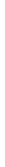
\includegraphics[max width=\linewidth, center]{external/whitespace-tikz/4cm.pdf}
\end{image}%
\end{project}
\end{document}